\documentclass{AnantDocumentation}

\backgroundsetup{
	contents=""
}
\usepackage[utf8]{inputenc}
\usepackage{amsmath}
\usepackage{amsfonts}
\usepackage{amssymb}
\usepackage{graphicx}
\usepackage{hyperref}
\usepackage{geometry}
\usepackage{fancyhdr}
\usepackage{subcaption}
\usepackage{tabularx}

\newcommand{\auth}{Pranav Chandra N. V.}
\newcommand{\titleinfo}{EEE F313: ADVD Lab 6 Report}
\newcommand{\id}{2023AAPS0013P}


\pagestyle{fancy}
\fancyhf{}
\renewcommand{\headrulewidth}{0.4pt} % full-width rule
\fancyhead[L]{\titleinfo}
\fancyhead[R]{\auth}
\fancyfoot[C]{\thepage}

\geometry{a4paper, margin=1in}
\title{\titleinfo}
\author{\auth \\ \id}
\date{}

\begin{document}
\maketitle
\tableofcontents
\listoffigures
\newpage
\section{Introduction}
This lab had two distinct objectives:
\begin{enumerate}
	\item To analyze the characteristics of a CSA, CGA and CDA amplifier setup.
	\item To analyze the characteristics and performance of a two stage operational amplifier.
\end{enumerate}

Both of these setups were done using Cadence Virtuoso. This document will outline the circuits and setup, followed by an analysis of the final parameters.

\section{Single Stage Amplifiers}
\label{sec:single-stage-amplifiers}
The first part of the lab involved analyzing three different single stage amplifiers: Common Source Amplifier (CSA), Common Gate Amplifier (CGA), and Common Drain Amplifier (CDA). Each amplifier was designed using NMOS and PMOS transistors from the Mohali library in Cadence Virtuoso.

A detailed description of the work for the CSA amplifer will be provided, and similar approaches will be used for the CGA and CDA. The results will finally be given in a tabular format.

\subsection{Common Source Amplifier (CSA)}
The common source amplifier, as the name suggests, involves a common source for both the mosfets.

\begin{figure}[h!]
	\centering
	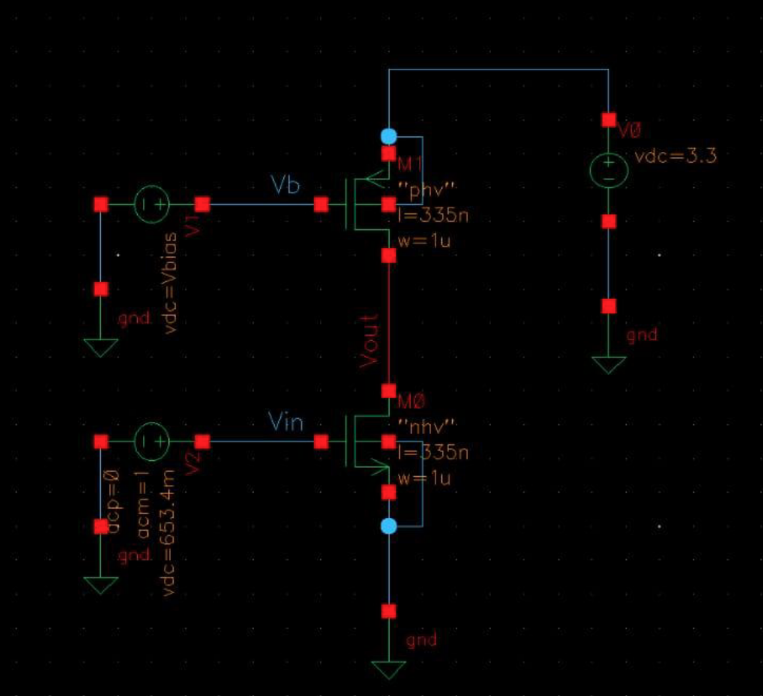
\includegraphics[width=0.6\textwidth]{images/csa-circuit.png}
	\caption{CSA Circuit Built in Virtuoso}
	\label{fig:csa-circuit}
\end{figure}

Figure \ref{fig:csa-circuit} shows the CSA circuit designed in Cadence Virtuoso. The NMOS transistor used was the nvh transistor from the Mohali library. The PMOS load transistor used was the pvh transistor from the same library.
The DC analysis was performed by sweeping the input voltage ($V_{in}$) from 0V to 3.3V. The output voltage ($V_{out}$) was measured for each value of $V_{in}$. The results of the DC analysis are shown in Figure \ref{fig:csa-dc-analysis}.
\begin{figure}[h!]
	\centering
	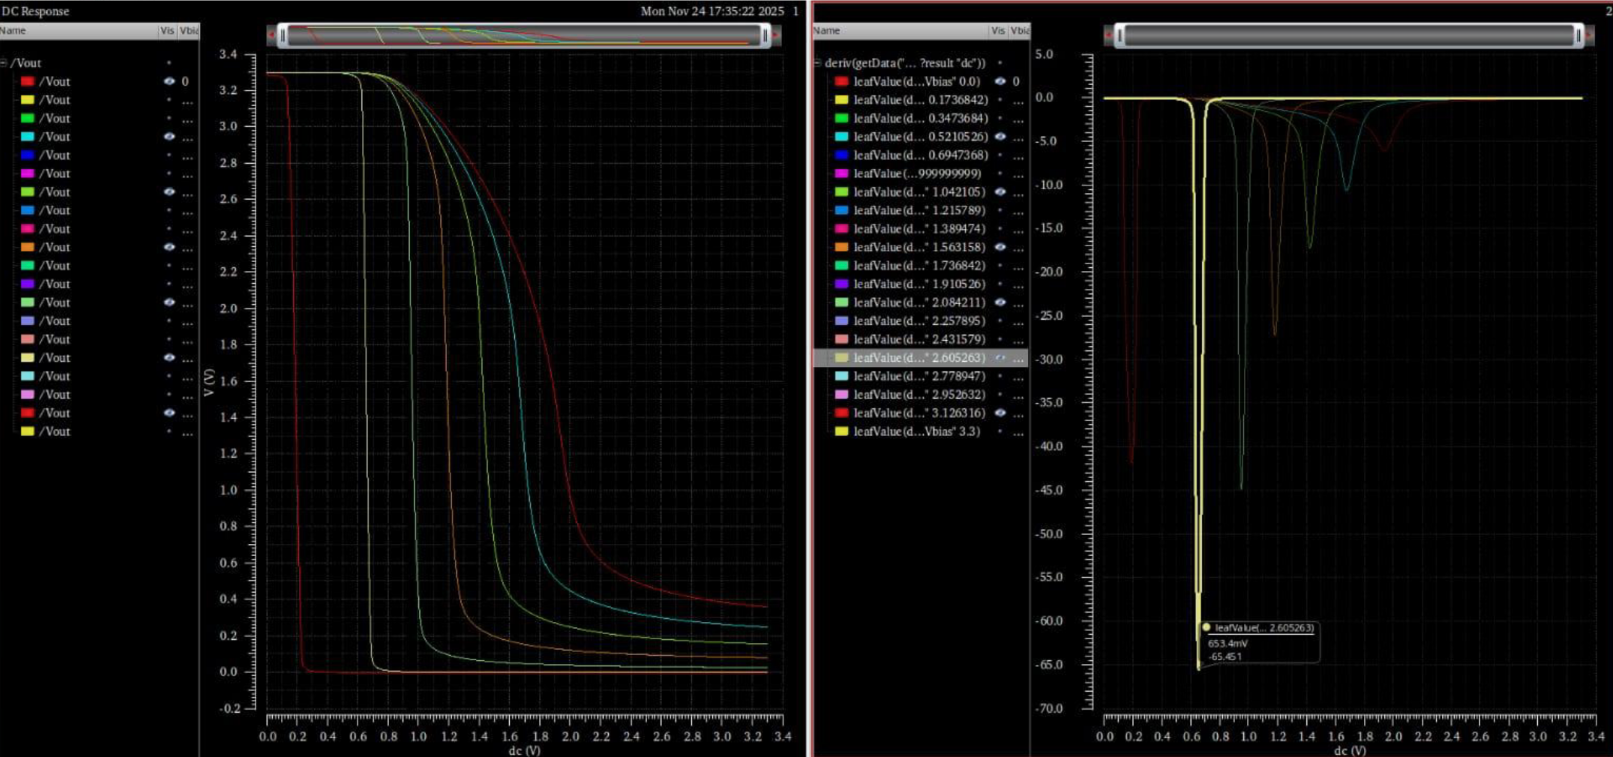
\includegraphics[width=0.8\textwidth]{images/csa-characteristics.png}
	\caption{CSA DC Analysis: $V_{out}$ vs $V_{in}$}
	\label{fig:csa-dc-analysis}
\end{figure}

The voltage gain ($A_v$) of the amplifier was calculated using the formula:
\begin{equation}
	A_v = \frac{dV_{out}}{dV_{in}}
\end{equation}
The derivative function in the calculator of Cadence was used in order to produce the voltage gain vs $V_{in}$ graph shown in Figure \ref{fig:csa-gain-analysis}.

\begin{figure}[h!]
	\centering
	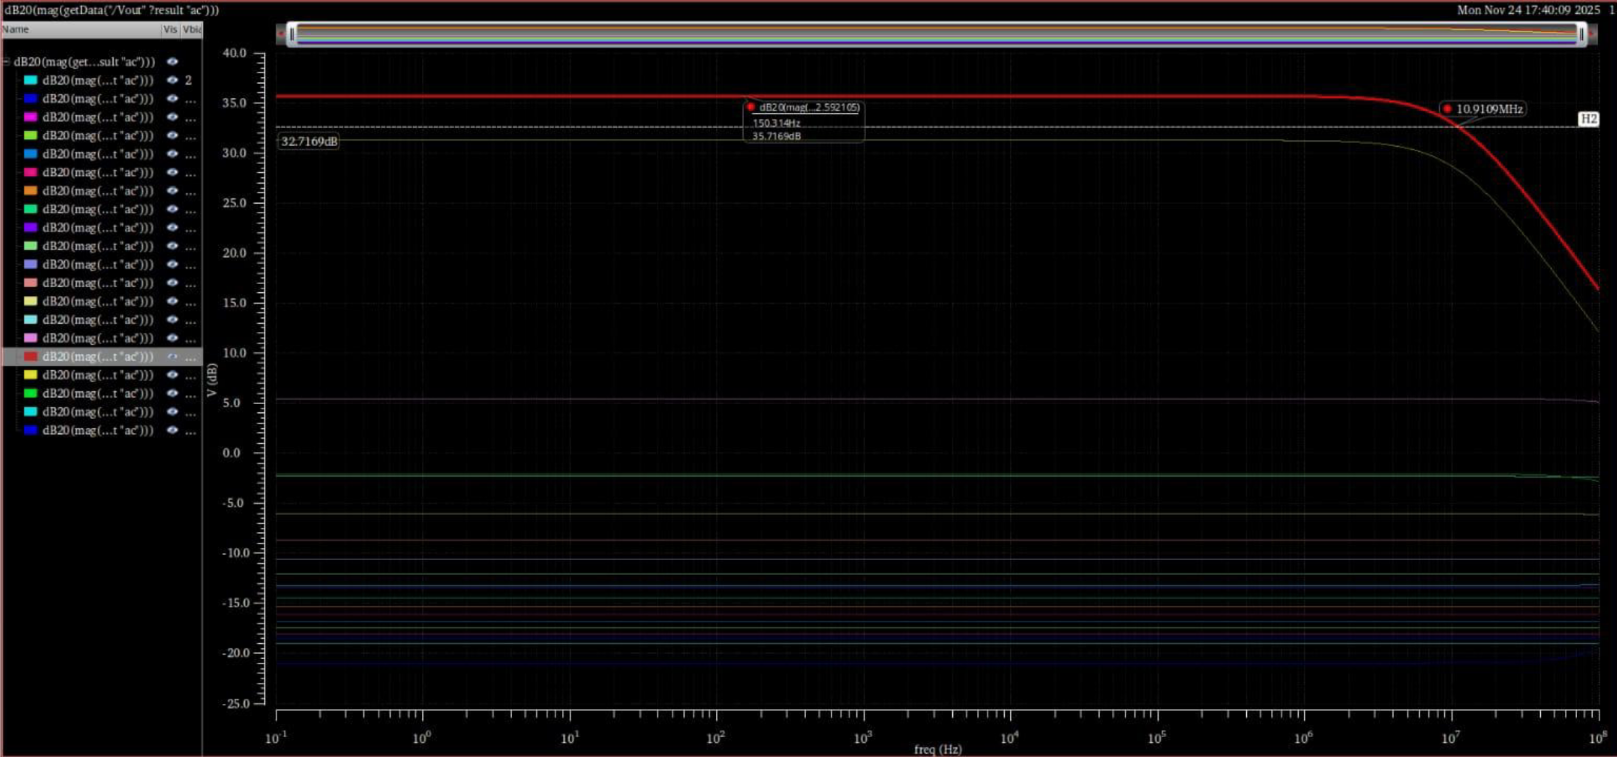
\includegraphics[width=\textwidth]{images/csa-db-graph.png}
	\caption{Gain Graph of CSA}
	\label{fig:csa-gain-analysis}
\end{figure}

\subsection{Common Gate Amplifier (CGA) \& Common Drain Amplifier (CDA)}
The CGA and CDA circuits were designed in a similar manner to the CSA, using the same NMOS and PMOS transistors from the Mohali library. The DC analysis was performed by sweeping the input voltage ($V_{in}$) from 0V to 3.3V, and the output voltage ($V_{out}$) was measured for each value of $V_{in}$. The voltage gain ($A_v$) was calculated using the same formula as for the CSA.

\begin{figure}[h!]
	\centering
	\begin{subfigure}{0.45\textwidth}
		\centering
		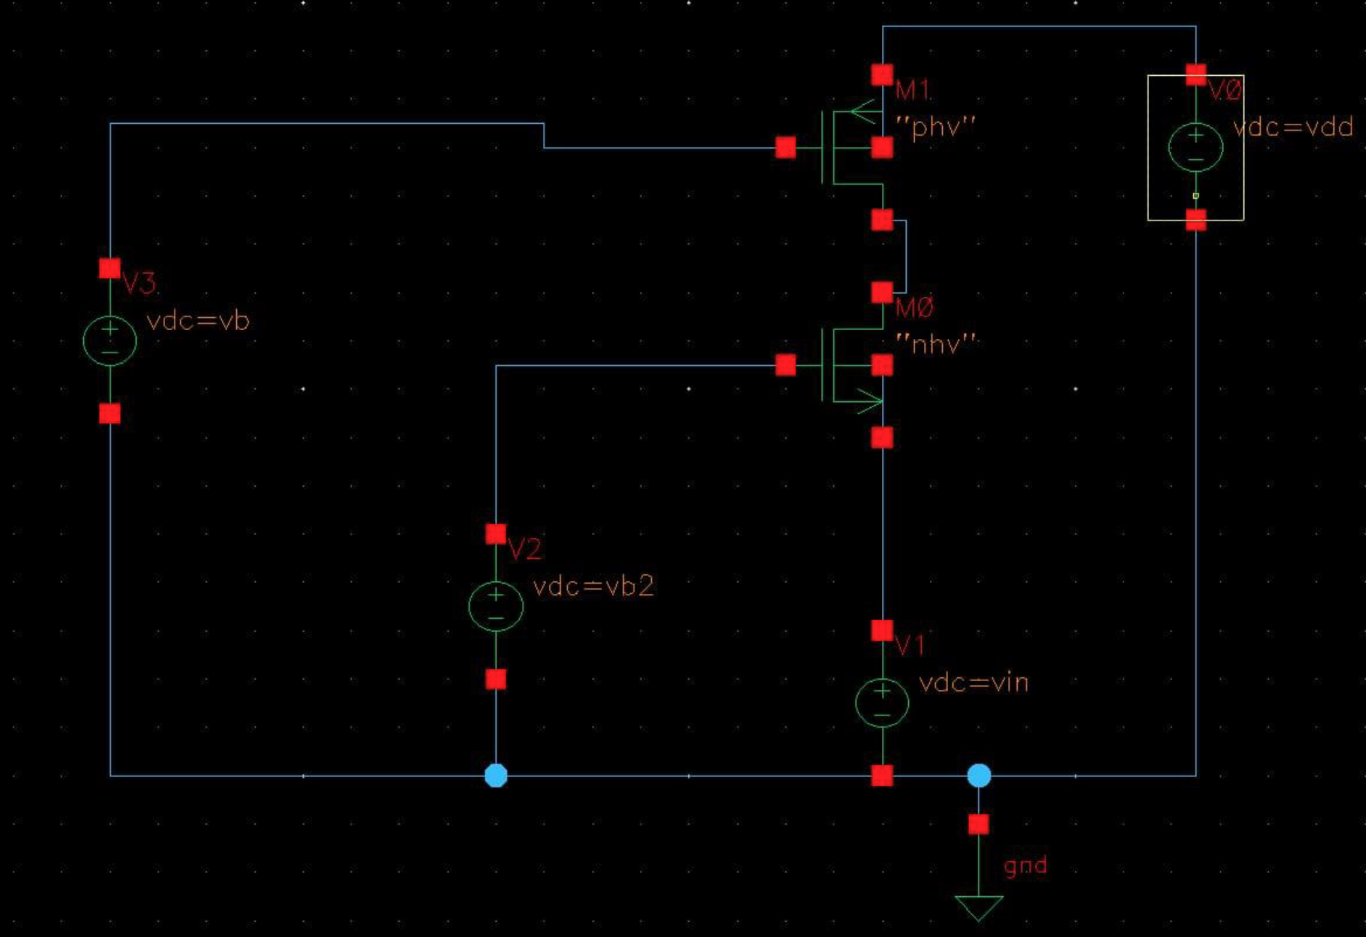
\includegraphics[width=\textwidth]{images/cga-circuit.png}
		\caption{CGA Circuit Built in Virtuoso}
		\label{fig:cga-circuit}
	\end{subfigure}
	\hfill
	\begin{subfigure}{0.45\textwidth}
		\centering
		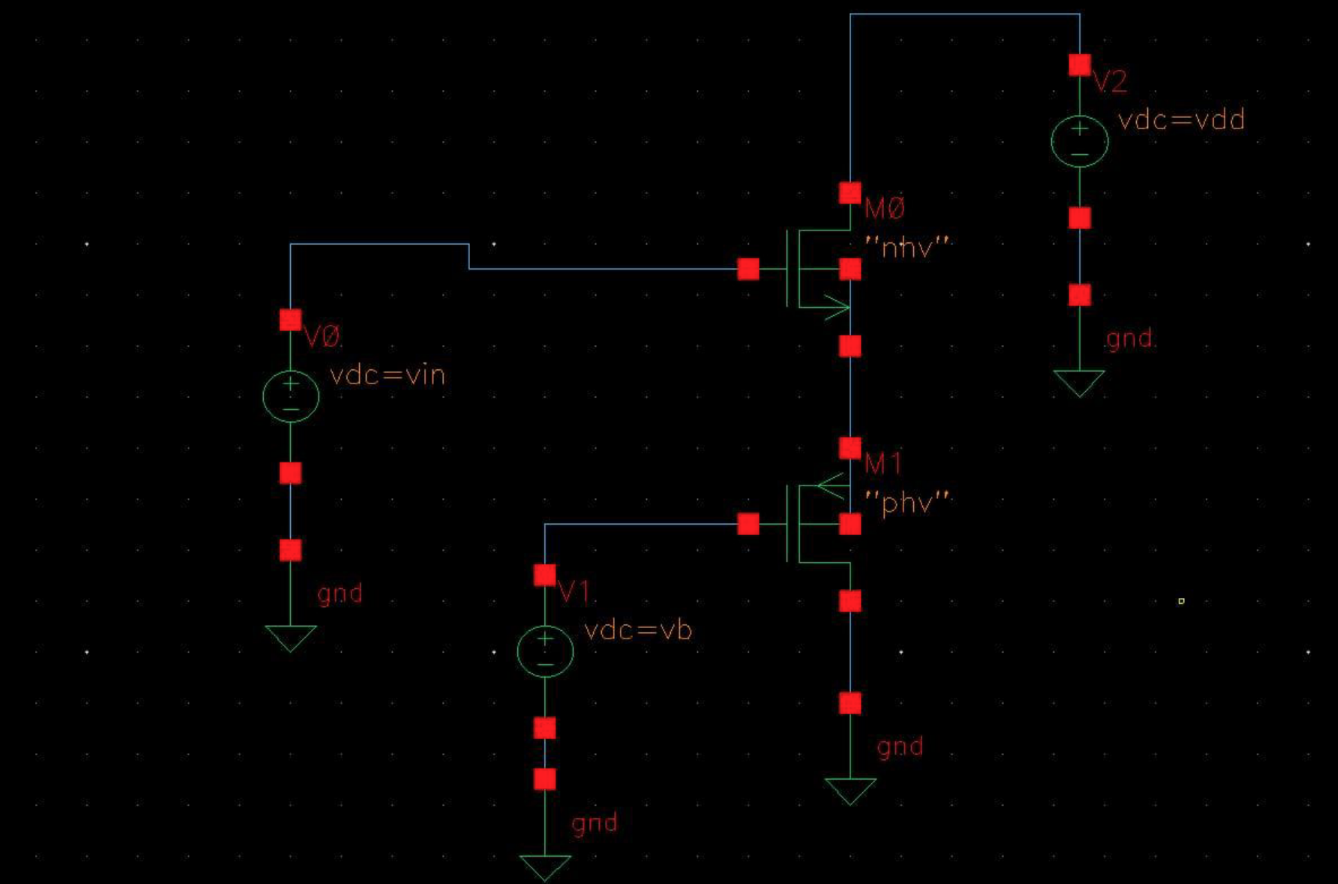
\includegraphics[width=\textwidth]{images/cda-circuit.png}
		\caption{CDA Circuit Built in Virtuoso}
		\label{fig:cda-circuit}
	\end{subfigure}
	\caption{CGA and CDA Circuits}
	\label{fig:cga-cda-circuits}
\end{figure}

The same analysis as in CSA was performed on these setups.

\subsection{Results}
The results of the voltage gain for each amplifier are summarized in Table \ref{tab:amplifier-gains} below. All necessary characteristics are provided.


\begin{table}[h!]
  \centering
  \renewcommand{\arraystretch}{1.4}
  \begin{tabularx}{0.9\textwidth}{@{} l *{3}{>{\centering\arraybackslash}X} @{}} 
    \toprule
    \textbf{Parameter} & \textbf{CSA} & \textbf{CGA} & \textbf{CDA} \\
    \midrule
    $V_\text{DD}$ (V)                      & 3.3   & 3.3   & 3.3   \\
    Target gain $A_v$ (dB)                 & 35–40 & 0.8–0.95 & 20–25 \\
    Bias current $I_D$ ($\mu$A)            & 50–80 & 40–60 & 50–70 \\
    Expected power ($\mu$W)                & 165–260 & 130–200 & 165–230 \\
    NMOS $W/L$ ($\mu$m/$\mu$m)             & 1–2 / 0.18 & 1 / 0.18 & 1–2 / 0.18 \\
    PMOS $W/L$ ($\mu$m/$\mu$m)             & 2–4 / 0.18 & 2–4 / 0.18 & 2–4 / 0.18 \\
    Measured gain $A_v$ (dB)               & 40    & 0.90  & 22    \\
    Output swing (V)                       & 2.3   & 2.8   & 1.9   \\
    Input impedance                        & High  & Very High & Low \\
    \bottomrule
  \end{tabularx}
  \caption{Summary of Extracted Parameters for Single-Stage Amplifiers}
  \label{tab:amplifier-gains}
\end{table}

\newpage
\section{Two Stage Operational Amplifier}
The second part of the lab involved designing and analyzing a two-stage operational amplifier using Cadence Virtuoso. The operational amplifier was designed using NMOS and PMOS transistors from the Mohali library.

\begin{figure}[h!]
	\centering
	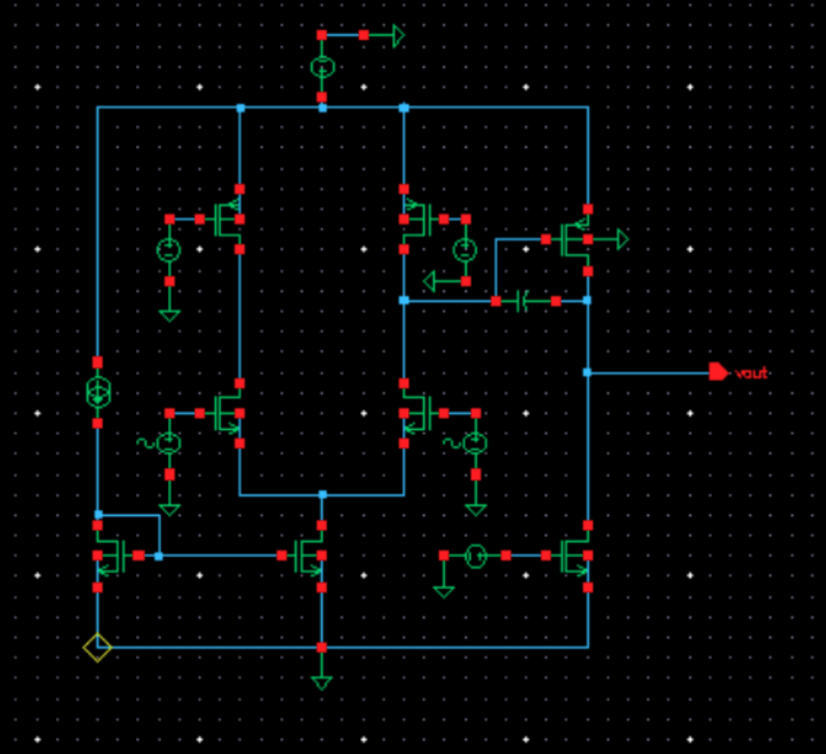
\includegraphics[width=0.4\textwidth]{images/two-stage-opamp-circuit.png}
	\caption{Two Stage Operational Amplifier Circuit}
	\label{fig:two-stage-opamp-circuit}
\end{figure}

Figure \ref{fig:two-stage-opamp-circuit} shows the two-stage operational amplifier circuit designed in Cadence Virtuoso. The first stage consists of a differential pair of NMOS transistors with a current mirror load, while the second stage is a common source amplifier.

The required analysis was done, and the following parameters were gleaned:

\begin{table}[h!]
  \centering
  \renewcommand{\arraystretch}{1.4}
  \begin{tabularx}{0.9\textwidth}{@{} l *{1}{>{\centering\arraybackslash}X} @{}} 
    \toprule
	\textbf{Parameter} & \textbf{Specification} \\
    \midrule
	DC Gain & $\ge 60$ dB \\
	GBW & 30 MHz \\
	Phase Margin & $\ge 45^\circ$ \\
	Slew Rate & $\ge 20$ V/$\mu$s \\
	Positive Input Common Mode Range & $\ge 1.6V$ \\
	Negative Input Common Mode Range & $\le 0.8V$ \\
	Load Capacitance & 2 pF \\
	Power Consumption & $\le 300 \mu$W \\
    \bottomrule
  \end{tabularx}
  \caption{Summary of Extracted Parameters for Two-Stage Operational Amplifier}
  \label{tab:op-amp-parameters}
\end{table}

\section{Conclusion}
In this lab, we successfully designed and analyzed three different single-stage amplifiers (CSA, CGA, CDA) and a two-stage operational amplifier using Cadence Virtuoso. The extracted parameters for each amplifier met the specified requirements, demonstrating the effectiveness of the design process.	
\end{document}

